\newpage
\chapter{METODE PENELITIAN} \label{Bab III}

\section{Alur Penelitian} \label{III.Alur}
Pada penelitian ini, tahapan pelaksanaan dirancang secara sistematis menggunakan pendekatan eksperimental kuantitatif komparatif untuk mengevaluasi kinerja, konsumsi sumber daya, serta ketahanan terhadap kegagalan dari tiga strategi \textit{event scheduling engine} (\textit{In-Memory Engine}, \textit{Database-Backed Worker}, dan \textit{Queue Engine}). Alur penelitian dimulai dari tahap studi literatur, perancangan arsitektur \textit{benchmarking testbed}, implementasi ketiga strategi beserta \textit{Push Notification Mock Server}, implementasi pembangkit beban (\textit{workload generator}) dan instrumentasi pemantauan, validasi lingkungan pengujian, eksekusi eksperimen pada berbagai skenario beban dan kegagalan, pengolahan serta analisis data hasil pengujian, hingga penyusunan rekomendasi pemilihan strategi. Secara keseluruhan, tahapan alur penelitian ini ditunjukkan dalam bentuk diagram alir (\textit{flowchart}) pada Gambar \ref{fig:3.alur}. \par

\begin{figure}[H] % Kalau menggunakan H, posisi gambar akan tepat dibawah teks
    \centering
    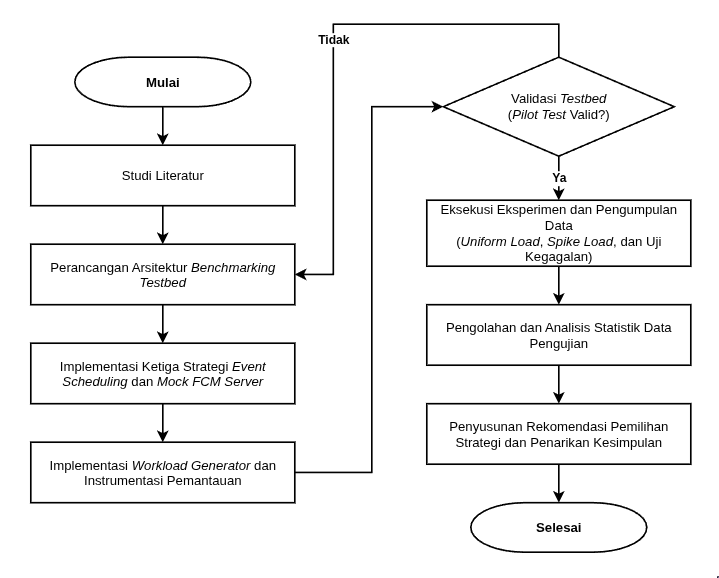
\includegraphics[width=0.6\textwidth]{figure/flowchart.png}
    \caption{Alur Penelitian}
    \label{fig:3.alur}
\end{figure}

\section{Penjabaran Langkah Penelitian} \label{III.Jabar Alur}
Jelaskan secara general langkah-langkah alur penelitian, yang sudah tergambar dalam flowchart di subbab \ref{III.Alur}. Subsubbab berikut harus sesuai dengan jumlah entitas langkah pada alur penelitian. \par

\subsection{Langkah 1} \label{III.Langkah 1}
Penjelasan Langkah 1. \par

\subsection{Langkah 2} \label{III.Langkah 2}
Penjelasan Langkah 2. \par

\section{Alat dan Bahan Tugas Akhir} \label{III.Alat dan Bahan}
Pada bagian ini dijabarkan perangkat keras, infrastruktur \textit{cloud}, perangkat lunak, serta bahan yang digunakan untuk membangun lingkungan pengujian dan menjalankan eksperimen. \par

\subsection{Alat} \label{III.Alat}
Alat yang digunakan dalam pelaksanaan penelitian ini terdiri atas perangkat keras atau infrastruktur \textit{Virtual Machine} pada satu \textit{Availability Zone} yang sama serta perangkat lunak pendukung sebagai berikut: \par
\begin{enumerate}[noitemsep]
	\item \textit{Virtual Machine} 1 (\textit{Workload Generator \& Monitoring Node}) dengan spesifikasi sistem operasi Ubuntu Server 24.04 LTS, \textit{dedicated processor} 2 vCPU (\textit{compute-optimized}, setara AWS \texttt{c6i.large} atau GCP \texttt{c2d-standard-2}), RAM 4 GB, dan penyimpanan SSD 30 GB untuk menjalankan pembangkit beban (\textit{producer}), Prometheus, serta Grafana.
	\item \textit{Virtual Machine} 2 (\textit{System Under Test / SUT Node}) dengan spesifikasi sistem operasi Ubuntu Server 24.04 LTS, \textit{dedicated processor} 4 vCPU (\textit{compute-optimized}, setara AWS \texttt{c6i.xlarge} atau GCP \texttt{c2d-standard-4}), RAM 8 GB, dan penyimpanan SSD 30 GB untuk menjalankan ketiga strategi \textit{event scheduling engine} beserta \textit{datastore} (PostgreSQL dan Redis) secara bergantian.
	\item \textit{Virtual Machine} 3 (\textit{Mock Server Node}) dengan spesifikasi sistem operasi Ubuntu Server 24.04 LTS, \textit{dedicated processor} 2 vCPU (\textit{compute-optimized}, setara AWS \texttt{c6i.large} atau GCP \texttt{c2d-standard-2}), RAM 4 GB, dan penyimpanan SSD 30 GB untuk menjalankan \textit{Push Notification Mock Server}.
	\item Bahasa pemrograman Go v1.26.3 beserta pustaka pendukung (\texttt{pgx/v5}, \texttt{asynq}, dan \texttt{gin-gonic/gin}).
	\item Sistem manajemen basis data relasional PostgreSQL v18 (Alpine) dan penyimpanan \textit{in-memory} Redis v8.8.2 (Alpine).
	\item \textit{Platform containerization} Docker dan Docker Compose untuk isolasi dan penyeragaman batas sumber daya komputasi.
	\item Perangkat pemantauan dan pengumpul metrik telemetri cAdvisor v0.51.0, Prometheus v3.13.3, dan Grafana v13.0.8.
	\item Layanan sinkronisasi waktu jaringan Chrony (NTP) untuk menyelaraskan jam sistem antar-\textit{Virtual Machine}.
	\item Perangkat pengolah data dan analisis statistik Python 3 beserta pustaka \texttt{pandas}, \texttt{scipy}, dan \texttt{matplotlib}.
	\item \textit{Code editor} dan sistem kendali versi Git serta GitHub.
\end{enumerate}

\subsection{Bahan} \label{III.Bahan}
Bahan yang digunakan dan diolah dalam penelitian ini adalah sebagai berikut: \par
\begin{enumerate}[noitemsep]
	\item Data beban kerja sintetis (\textit{synthetic workload dataset}) pihak pertama yang dibangkitkan secara terprogram melalui \textit{workload generator} sesuai pola distribusi \textit{uniform load} dan \textit{spike load}, berisi atribut identitas tugas (\texttt{project\_id}, \texttt{token}), isi pesan (\texttt{title}, \texttt{body}), serta target waktu eksekusi (\texttt{scheduled\_at}).
	\item Dokumen spesifikasi protokol dan struktur \textit{payload} antarmuka Firebase Cloud Messaging (FCM) HTTP v1 API sebagai acuan perancangan \textit{Push Notification Mock Server}.
	\item Literatur ilmiah, buku teks, dan artikel rujukan terkait algoritma penjadwalan waktu nyata, arsitektur antrean terdistribusi, serta mekanisme konkurensi basis data yang disitasi pada penelitian ini.
\end{enumerate}

\section{Metode Pengembangan} \label{III.Metode}
Membahas mengenai metode yang digunakan dalam penelitian, berdasarkan dasar teori yang sebelumnya sudah dijelaskan pada subbab \ref{II.Teori}. Setiap Tugas Akhir wajib memiliki metode dalam pelaksanaannya yang sesuai dengan penelitian yang dikerjakan: \par
\begin{enumerate}[noitemsep]
	\item Alur pengembangan tugas akhir, menggunakan flowchart
	\item Cara pengumpulan data yang digunakan (Kuesioner, Wawancara, pengujian, dan lainnya)
	\item Metode pengembangan tugas akhir (Metode Waterfall, Agile, RAD, dan lainnya).
	\item Metode pengujian penelitian
\end{enumerate}
Subbab ini akan berhubungan erat dengan Bab \ref{Bab IV}. \par

\section{Ilustrasi Perhitungan Metode} \label{III.Ilustrasi}
Penjelasan contoh perhitungan bagi penelitian tugas akhir yang menggunakan algoritma perhitungan tertentu. Rumus perhitungan berdasarkan rumus yang sudah dijelaskan sebelumnya di Bab \ref{II.Teori}. \par

\section{Rancangan Pengujian} \label{III.Rancang_Uji}
Penjabaran terkait rancangan pengujian, pengujian perangkat keras, lunak, fungsional, dan non-fungsional. Berikan juga hipotesis hasil yang diharapkan dari penelitian. \par
